\chapter{Aplicando a Diagonaliza\c{c}\~ao de Ursin}\label{sec.diagonalizacao_ursin}

%\section{Introdu\c{c}\~ao}
   

\section{Aplicando a Diagonaliza\c{c}\~ao de Ursin na Equa\c{c}\~ao \ref{eq.matricial_1}}\label{sec.diagonalizacao_1}

Comparando a equa\c{c}\~ao \ref{eq.matricial_1} com a equa\c{c}\~ao \ref{eq.matricial} vemos que as matrizes
\begin{equation*}
M^{(1)}_1=\frac{-\mu_0\sigma-i\,\gamma^2\omega}{\overline{\sigma}}\qquad\text{e}\qquad\,M^{(1)}_2=\frac{\overline{\sigma}}{i\,\omega}.
\end{equation*}
Definimos autovalores e autovetores relacionados ao operador $M^{(1)}_1\cdot M^{(1)}_2$ na forma 
\begin{equation}\label{eq.def_auto_1}
\frac{-\mu_0\sigma-i\,\gamma^2\omega}{\overline{\sigma}}\cdot\frac{\overline{\sigma}}{i\,\omega}\,\mathbf{a}^{(1)}={q^{(1)}}^2\mathbf{a}^{(1)},
\end{equation}
e para termos um autovetor n\~ao trivial, \'e necess\'ario o autovalor
\begin{equation*}
q^{(1)}=\sqrt{\frac{-\mu_0\sigma-i\,\gamma^2\omega}{i\,\omega}}.
\end{equation*}
Substituindo o autovalor acima na equa\c{c}\~ao \ref{eq.def_auto_1}, temos que o autovetor $\mathbf{a}^{(1)}$ \'e o autoespa\c{c}o relativo ao autovalor $q^{(1)}$ e ${1}$ \'e uma base para esse autoespa\c{c}o.\\
O autovetor relacionado ao operador $M^{(1)}_2\cdot M^{(1)}_1$ \'e dado por
\begin{equation*}
\mathbf{b}^{(1)}=\frac{\overline{\sigma}}{i\,\omega\,\sqrt{\frac{-\mu_0\sigma-i\,\gamma^2\omega}{i\,\omega}}}\cdot\mathbf{a}^{(1)}.
\end{equation*}
Tomando arbitrariamente o valor $\mathbf{a}^{(1)}=1$ temos que as submatrizes de diagonaliza\c{c}\~ao s\~ao
\begin{equation*}
L^{(1)}_1=1\qquad\text{e}\qquad L^{(1)}_2=\frac{\overline{\sigma}}{i\,\omega\,\sqrt{\frac{-\mu_0\sigma-i\,\gamma^2\omega}{i\,\omega}}},
\end{equation*}
e as matrizes para diagonaliza\c{c}\~ao s\~ao dadas por
\begingroup
\Large
\begin{align*}
L^{(1)}&=\frac{1}{\sqrt{2}}\,
\begin{pmatrix}
1&1\\
\frac{\overline{\sigma}}{i\,\omega\,\sqrt{\frac{-\mu_0\sigma-i\,\gamma^2\omega}{i\,\omega}}}&-\frac{\overline{\sigma}}{i\,\omega\,\sqrt{\frac{-\mu_0\sigma-i\,\gamma^2\omega}{i\,\omega}}}
\end{pmatrix}\\\\
{L^{(1)}}^{-1}&=\frac{1}{\sqrt{2}}\,
\begin{pmatrix}
1&\frac{i\,\omega\,\sqrt{\frac{-\mu_0\sigma-i\,\gamma^2\omega}{i\,\omega}}}{\overline{\sigma}}\\
1&-\frac{i\,\omega\,\sqrt{\frac{-\mu_0\sigma-i\,\gamma^2\omega}{i\,\omega}}}{\overline{\sigma}}
\end{pmatrix}.
\end{align*}
\endgroup
A matriz semelhante a $M^{(1)}$ \'e
\begin{equation*}
\tilde{\Lambda}^{(1)}=
\begin{pmatrix}
\sqrt{\frac{-\mu_0\sigma-i\,\gamma^2\omega}{i\,\omega}}&0\\
0&-\sqrt{\frac{-\mu_0\sigma-i\,\gamma^2\omega}{i\,\omega}}
\end{pmatrix}.
\end{equation*}

\section{Aplicando a Diagonaliza\c{c}\~ao de Ursin na Equa\c{c}\~ao \ref{eq.matricial_2}}\label{sec.diagonalizacao_2}

Comparando a equa\c{c}\~ao \ref{eq.matricial_2} com a equa\c{c}\~ao \ref{eq.matricial} vemos que as matrizes
\begin{equation*}
M^{(2)}_1=-\mu_0\qquad\text{e}\qquad\,M^{(2)}_2=\frac{\overline{\sigma}\,\mu_0+i\,\omega\,\gamma^2}{i\,\omega\,\mu_0}.
\end{equation*}
Definimos autovalores e autovetores relacionados ao operador $M^{(2)}_1\cdot M^{(2)}_2$ na forma
\begin{equation}\label{eq.def_auto_2}
-\mu_0\cdot\frac{\overline{\sigma}\,\mu_0+i\,\omega\,\gamma^2}{i\,\omega\,\mu_0}\,\mathbf{a}^{(2)}={q^{(2)}}^2\mathbf{a}^{(2)},
\end{equation}
e para termos um autovetor n\~ao trivial, \'e necess\'ario o autovalor
\begin{equation*}
q^{(2)}=\sqrt{-\frac{\overline{\sigma}\,\mu_0+i\,\omega\,\gamma^2}{i\,\omega}}.
\end{equation*}
Substituindo o autovalor $q^{(2)}$ na equa\c{c}\~ao \ref{eq.def_auto_2}, temos que o autovetor $\mathbf{a}^{(2)}$ \'e o autoespa\c{c}o relativo ao autovalor $q^{(2)}$ e ${1}$ \'e uma base para esse autoespa\c{c}o.\\
O autovetor relacionado ao operador $M^{(2)}_2\cdot M^{(2)}_1$ \'e dado por
\begin{equation*}
\mathbf{b}^{(2)}=-\frac{1}{\mu_0}\,\sqrt{-\frac{\overline{\sigma}\,\mu_0+i\,\omega\,\gamma^2}{i\,\omega}}\cdot\mathbf{a}^{(2)}.
\end{equation*}
Tomando arbitrariamente o valor $\mathbf{a}^{(2)}=1$ temos que as submatrizes de diagonaliza\c{c}\~ao s\~ao
\begin{equation*}
L^{(2)}_1=1\qquad\text{e}\qquad L^{(2)}_2=-\frac{1}{\mu_0}\,\sqrt{-\frac{\overline{\sigma}\,\mu_0+i\,\omega\,\gamma^2}{i\,\omega}},
\end{equation*}
e as matrizes para diagonaliza\c{c}\~ao s\~ao dadas por
\begin{Large}
\begin{align*}
L^{(2)}&=\frac{1}{\sqrt{2}}\,
\begin{pmatrix}
1&1\\
-\frac{1}{\mu_0}\,\sqrt{-\frac{\overline{\sigma}\,\mu_0+i\,\omega\,\gamma^2}{i\,\omega}}&\frac{1}{\mu_0}\,\sqrt{-\frac{\overline{\sigma}\,\mu_0+i\,\omega\,\gamma^2}{i\,\omega}}
\end{pmatrix}\\\\
{L^{(2)}}^{-1}&=\frac{1}{\sqrt{2}}\,
\begin{pmatrix}
1&-\mu_0\,(-\frac{\overline{\sigma}\,\mu_0+i\,\omega\,\gamma^2}{i\,\omega})^{-\frac{1}{2}}\\
1&\mu_0\,(-\frac{\overline{\sigma}\,\mu_0+i\,\omega\,\gamma^2}{i\,\omega})^{-\frac{1}{2}}
\end{pmatrix}.
\end{align*}
\end{Large}
A matriz semelhante a $M^{(2)}$ \'e
\begin{equation*}
\tilde{\Lambda}^{(2)}=
\begin{pmatrix}
\sqrt{-\frac{\overline{\sigma}\,\mu_0+i\,\omega\,\gamma^2}{i\,\omega}}&0\\
0&-\sqrt{-\frac{\overline{\sigma}\,\mu_0+i\,\omega\,\gamma^2}{i\,\omega}}
\end{pmatrix}.
\end{equation*}

\section{Aplicando a Diagonaliza\c{c}\~ao de Ursin na Equa\c{c}\~ao \ref{eq.matricial_3}}\label{sec.diagonalizacao_3}

Comparando a equa\c{c}\~ao \ref{eq.matricial_3} com a equa\c{c}\~ao \ref{eq.matricial} vemos que as matrizes
\begin{equation*}
M^{(3)}_1=
\begin{pmatrix}
\beta&\lambda\,\gamma\,\beta\\
\lambda\,\gamma\,\beta&\rho+\gamma^2\beta(\lambda^2-\beta^{-1})
\end{pmatrix}
\quad\text{e}\quad
M^{(3)}_2=
\begin{pmatrix}
\rho&\gamma\\
\gamma&G^{-1}
\end{pmatrix}
\end{equation*}
onde definimos $\beta=\frac{1}{\lambda+2\,G}$.\\
Definimos autovalores e autovetores relacionados ao operador $M^{(3)}_1\cdot M^{(3)}_2$ na forma
\begin{equation*}
\begin{pmatrix}
\beta&\lambda\,\gamma\,\beta\\
\lambda\,\gamma\,\beta&\rho+\gamma^2\beta(\lambda^2-\beta^{-1})
\end{pmatrix}
\cdot
\begin{pmatrix}
\rho&\gamma\\
\gamma&G^{-1}
\end{pmatrix}
\,\mathbf{a}^{(3)}_i
=
{q^{(3)}_i}^2\mathbf{a}^{(3)}_i,
\end{equation*}
para $i=1,2$.  E para evitarmos solu\c{c}\~oes triviais, \'e necess\'ario que seja nulo o determinante da matriz
\begin{equation}\label{eq.def_auto_3}
\begin{pmatrix}
\beta\,\rho+\lambda\,\gamma^2\beta-{q^{(3)}_i}^2&\beta\,\gamma+\lambda\,\gamma\,\beta\,G^{-1}\\
\lambda\,\gamma\,\beta\,\rho+\rho\,\gamma+\gamma^3\beta\,(\lambda^2-\beta^{-2})&\lambda\,\gamma^2\beta+\frac{\rho+\gamma^2\beta\,(\lambda^2-\beta^{-2})}{G}-{q^{(3)}_i}^2
\end{pmatrix}
\begin{pmatrix}
a_{i\,1}\\
a_{i\,2}
\end{pmatrix}
=
\begin{pmatrix}
0\\
0
\end{pmatrix}.
\end{equation}
Anulando o determinante da matriz acima chegamos \`a equa\c{c}\~ao do segundo grau em ${q^{(3)}_i}^2$
\begin{equation*}
\begin{split}
{q^{(3)}_i}^4-\left(\beta\,\rho+2\,\lambda\,\gamma^2\beta+\frac{\rho+\gamma^2\beta\,(\lambda^2-\beta^{-2})}{G}\right)\,{q^{(3)}_i}^2\\\\
-\left(\beta\,\gamma+\lambda\,\gamma\,\beta\,G^{-1}\right)\left[\lambda\,\gamma\,\beta\,\rho+\rho\,\gamma+\gamma^3\beta\,(\lambda^2-\beta^{-2})\right]\\\\
+(\beta\,\rho+\lambda\,\gamma^2\beta)\left[\lambda\,\gamma^2\beta+\frac{\rho+\gamma^2\beta\,(\lambda^2-\beta^{-2})}{G}\right]=0.
\end{split}
\end{equation*}
Os autovalores ${q^{(3)}_1}^2$ e ${q^{(3)}_2}^2$ s\~ao dados, respectivamente, tomando o sinal positivo e o sinal negativo antes da radicia\c{c}\~ao na equa\c{c}\~ao
\begin{equation*}
{q^{(3)}_i}^2=\frac{1}{2}\,\left[\beta\,\rho+2\,\lambda\,\gamma^2\beta+\frac{\rho+\gamma^2\beta\,(\lambda^2-\beta^{-2})}{G}\right]\pm\frac{1}{2}\sqrt{\Delta},
\end{equation*}
onde $\Delta$ \'e dado por
\begin{align*}
\Delta&=
\left[\beta\,\rho+2\,\lambda\,\gamma^2\beta+\frac{\rho+\gamma^2\beta\,(\lambda^2-\beta^{-2})}{G}\right]^2\\\\
&-4\,(\beta\,\rho+\lambda\,\gamma^2\beta)\left[\lambda\,\gamma^2\beta+\frac{\rho+\gamma^2\beta\,(\lambda^2-\beta^{-2})}{G}\right]\\\\
&+4\,\left(\beta\,\gamma+\lambda\,\gamma\,\beta\,G^{-1}\right)\left[\lambda\,\gamma\,\beta\,\rho+\rho\,\gamma+\gamma^3\beta\,(\lambda^2-\beta^{-2})\right].
\end{align*}
Como ${q^{(3)}_i}^2$ foi deduzido de forma que a matriz na equa\c{c}\~ao \ref{eq.def_auto_3} tenha determinante nulo, temos que as linhas dessa matriz s\~ao linearmente dependentes. Assim, vamos utilizar a linha 1 para definir os autovetores
\begin{equation*}
a_{i1}=-\frac{\beta\,\gamma+\lambda\,\gamma\,\beta\,G^{-1}}{\beta\,\rho+\lambda\,\gamma^2\beta-{q^{(3)}_i}^2}\,a_{i2},
\end{equation*}
onde $a_{i2}\in \mathbb{C}$. Por quest\~ao de facilidade de escrita, dentro do autoespa\c{c}o definido pela equa\c{c}\~ao acima, vamos escolher $a_{i2}=\beta\,\rho+\lambda\,\gamma^2\beta-{q^{(3)}_i}^2$, e os autovetores relacionados ao operador $M^{(3)}_1\cdot M^{(3)}_2$ s\~ao
\begin{equation*}
\mathbf{a}^{(3)}_1
=
\begin{pmatrix}
-\beta\,\gamma+\lambda\,\gamma\,\beta\,G^{-1}\\
\beta\,\rho+\lambda\,\gamma^2\beta-{q^{(3)}_1}^2
\end{pmatrix}
\quad\text{e}\quad
\mathbf{a}^{(3)}_2
=
\begin{pmatrix}
-\beta\,\gamma+\lambda\,\gamma\,\beta\,G^{-1}\\
\beta\,\rho+\lambda\,\gamma^2\beta-{q^{(3)}_2}^2
\end{pmatrix}.
\end{equation*}
Os autovetores relacionados ao operador $M^{(3)}_2\cdot M^{(3)}_1$ s\~ao dados por
\begin{align*}
\mathbf{b}^{(3)}_1
&=
\frac{1}{{q^{(3)}_1}}
\begin{pmatrix}
-\rho\,(\beta\,\gamma+\lambda\,\gamma\,\beta\,G^{-1})+\gamma\,(\beta\,\rho+\lambda\,\gamma^2\beta-{q^{(3)}_1}^2)\\
-\gamma\,(\beta\,\gamma+\lambda\,\gamma\,\beta\,G^{-1})+G^{-1}(\beta\,\rho+\lambda\,\gamma^2\beta-{q^{(3)}_1}^2)
\end{pmatrix}\\\\
\mathbf{b}^{(3)}_2
&=
\frac{1}{{q^{(3)}_2}}
\begin{pmatrix}
-\rho\,(\beta\,\gamma+\lambda\,\gamma\,\beta\,G^{-1})+\gamma\,(\beta\,\rho+\lambda\,\gamma^2\beta-{q^{(3)}_2}^2)\\
-\gamma\,(\beta\,\gamma+\lambda\,\gamma\,\beta\,G^{-1})+G^{-1}(\beta\,\rho+\lambda\,\gamma^2\beta-{q^{(3)}_2}^2)
\end{pmatrix}.
\end{align*}
Usando os autovetores, temos que as submatrizes de diagonaliza\c{c}\~ao s\~ao
\begin{equation*}
L^{(3)}_1=
\begin{pmatrix}
\mathbf{a}^{(3)}_1&\mathbf{a}^{(3)}_2
\end{pmatrix}
\quad\text{e}\quad
L^{(3)}_2=
\begin{pmatrix}
\mathbf{b}^{(3)}_1&\mathbf{b}^{(3)}_2
\end{pmatrix},
\end{equation*}
e as matrizes para diagonaliza\c{c}\~ao s\~ao dadas por
\begin{align*}
L^{(3)}&=\frac{1}{\sqrt{2}}
\begin{pmatrix}
\mathbf{a}^{(3)}_1&\mathbf{a}^{(3)}_2&\mathbf{a}^{(3)}_1&\mathbf{a}^{(3)}_2\\
\mathbf{b}^{(3)}_1&\mathbf{b}^{(3)}_2&-\mathbf{b}^{(3)}_1&-\mathbf{b}^{(3)}_2
\end{pmatrix}
\quad\text{e}
\\\\
{L^{(3)}}^{-1}&=\frac{1}{\sqrt{2}}
\begin{pmatrix}
{\mathbf{b}^{(3)}_1}^{\top}&{\mathbf{a}^{(3)}_1}^{\top}\\
{\mathbf{b}^{(3)}_2}^{\top}&{\mathbf{a}^{(3)}_2}^{\top}\\
{\mathbf{b}^{(3)}_1}^{\top}&-{\mathbf{a}^{(3)}_1}^{\top}\\
{\mathbf{b}^{(3)}_2}^{\top}&-{\mathbf{a}^{(3)}_2}^{\top}
\end{pmatrix}.
\end{align*}
A matriz semelhante a $M^{(3)}$ \'e
\begin{equation*}
\tilde{\Lambda}^{(3)}=
\begin{pmatrix}
q^{(3)}_1&0&0&0\\
0&q^{(3)}_2&0&0\\
0&0&-q^{(3)}_1&0\\
0&0&0&-q^{(3)}_2
\end{pmatrix}.
\end{equation*}


\section{Aplicando a Diagonaliza\c{c}\~ao de Ursin na Equa\c{c}\~ao \ref{eq.matricial_4}}\label{sec.diagonalizacao_4}

Comparando a equa\c{c}\~ao \ref{eq.matricial_4} com a equa\c{c}\~ao \ref{eq.matricial} vemos que as matrizes
\begin{equation*}
M^{(4)}_1=G^{-1}\qquad\text{e}\qquad\,M^{(4)}_2=\rho-G\,\gamma^2.
\end{equation*}
Definimos autovalores e autovetores relacionados ao operador $M^{(4)}_1\cdot M^{(4)}_2$ na forma
\begin{equation}\label{eq.def_auto_4}
G^{-1}(\rho-G\,\gamma^2)\,\mathbf{a}^{(4)}={q^{(4)}}^2\mathbf{a}^{(4)},
\end{equation}
e para termos um autovetor n\~ao trivial, \'e necess\'ario o autovalor
\begin{equation*}
{q^{(4)}}^2=G^{-1}(\rho-G\,\gamma^2).
\end{equation*}
Substituindo o autovalor ${q^{(4)}}^2$ na equa\c{c}\~ao \ref{eq.def_auto_4}, temos que o autovetor $\mathbf{a}^{(4)}$ \'e o autoespa\c{c}o relativo ao autovalor ${q^{(4)}}^2$ e ${1}$ \'e uma base para esse autoespa\c{c}o.\\
O autovetor relacionado ao operador $M^{(4)}_2\cdot M^{(4)}_1$ \'e dado por
\begin{equation*}
\mathbf{b}^{(4)}=[G\,(\rho-G\,\gamma^2)]^{\frac{1}{2}}   \cdot\mathbf{a}^{(4)}.
\end{equation*}
Tomando arbitrariamente o valor $\mathbf{a}^{(4)}=1$ temos que as submatrizes de diagonaliza\c{c}\~ao s\~ao
\begin{equation*}
L^{(4)}_1=1\qquad\text{e}\qquad L^{(4)}_2=[G\,(\rho-G\,\gamma^2)]^{\frac{1}{2}},
\end{equation*}
e as matrizes para diagonaliza\c{c}\~ao s\~ao dadas por
\begin{align*}
L^{(4)}&=\frac{1}{\sqrt{2}}\,
\begin{pmatrix}
1&1\\
[G\,(\rho-G\,\gamma^2)]^{\frac{1}{2}}&-[G\,(\rho-G\,\gamma^2)]^{\frac{1}{2}}
\end{pmatrix}\\\\
{L^{(4)}}^{-1}&=\frac{1}{\sqrt{2}}\,
\begin{pmatrix}
1&[G\,(\rho-G\,\gamma^2)]^{-\frac{1}{2}}\\
1&-[G\,(\rho-G\,\gamma^2)]^{-\frac{1}{2}}
\end{pmatrix}.
\end{align*}
A matriz semelhante a $M^{(4)}$ \'e
\begin{equation*}
\tilde{\Lambda}^{(4)}=
\begin{pmatrix}
[G^{-1}(\rho-G\,\gamma^2)]^{\frac{1}{2}}&0\\
0&-[G^{-1}(\rho-G\,\gamma^2)]^{\frac{1}{2}}
\end{pmatrix}.
\end{equation*}





%\section{Decomposi\c{c}\~ao em Ondas Ascendentes e Descentes}
%
%Para realizar a decomposi\c{c}\~ao do vetor $\mathbf{B}$ em ondas ascendentes e descendentes aplicamos uma diagonaliza\c{c}\~ao em autovalores na matriz $A$ na forma
%\begin{equation}\label{eq.diagonalizacao}
%A=L\,\Lambda_1L^{-1}\,,
%\end{equation}
%onde $\Lambda_1$ \'e a matriz diagonal dos autovalores $\lambda_i$ para $i=1,2,...,n$, e $L$ \'e a matriz dos autovetores correspondentes,
%\begin{equation}\label{eq.Lambda_1}
%\Lambda_1=
%\begin{bmatrix}
%\Lambda&0\\
%0&-\Lambda
%\end{bmatrix}\,.
%\end{equation} 
%A defini\c{c}\~ao de autovalores e autovetores \'e dada por
%\begin{equation}\label{eq.sist_autovalores}
%\begin{bmatrix}
%0&A_1\\
%A_2&0
%\end{bmatrix}
%\begin{bmatrix}
%\mathbf{L_1}\\
%\mathbf{L_2}
%\end{bmatrix}
%=
%\lambda\,
%\begin{bmatrix}
%\mathbf{L_1}\\
%\mathbf{L_2}
%\end{bmatrix}
%\end{equation}
%e aplicando o procedimento
%\begin{equation*}
%\begin{bmatrix}
%0&A_1\\
%A_2&0
%\end{bmatrix}
%\begin{bmatrix}
%0&A_1\\
%A_2&0
%\end{bmatrix}
%\begin{bmatrix}
%\mathbf{L_1}\\
%\mathbf{L_2}
%\end{bmatrix}
%=
%\lambda\,\lambda\,
%\begin{bmatrix}
%\mathbf{L_1}\\
%\mathbf{L_2}
%\end{bmatrix}\,,
%\end{equation*}
%podemos separar o sitema \ref{eq.sist_autovalores} de dimens\~ao $2n$ em dois sistemas de dimens\~ao n
%\begin{align*}
%A_1A_2\mathbf{L_1}&=\lambda^2\mathbf{L_1}\\
%A_2A_1\mathbf{L_2}&=\lambda^2\mathbf{L_2}\,,
%\end{align*}
%onde $\mathbf{L}_i$ s\~ao os vetores que, concatenados dois a dois, formam os autovetores que comp\~oem $L$.
%Assim, podemos dividir a diagonaliza\c{c}\~ao dada em \ref{eq.diagonalizacao} em duas diagonaliza\c{c}\~oes de dimens\~ao $n$
%\begin{align}\label{eq.subdiagonalizacao}\nonumber
%A_1A_2&=L_1\Lambda^2L_1^{-1}\\\quad\\\nonumber
%A_2A_1&=L_2\Lambda^2L_2^{-1}\,,
%\end{align}
%onde $L_i$ s\~ao submatrizes da matriz $L$ e cont\^em os autovetores $\mathbf{L}_i$.
%
%
%
%Definindo a matriz 
%\begin{equation}\label{eq.L}
%L=\frac{1}{\sqrt{2}}
%\begin{bmatrix}
%L_1&L_1\\
%L_2&-L_2
%\end{bmatrix}
%\end{equation}
%e sua inversa
%\begin{equation}\label{eq.L_inversa}
%L^{-1}=\frac{1}{\sqrt{2}}
%\begin{bmatrix}
%L_1^{-1}&L_2^{-1}\\
%L_1^{-1}&-L_2^{-1}
%\end{bmatrix}\,,
%\end{equation}
%podemos substitu\'i-las na equa\c{c}\~ao \ref{eq.diagonalizacao} e verificar que 
%\begin{align}\label{eq.definicao_A1_A2}\nonumber
%A_1&=L_1\Lambda\,L_2^{-1}\\\quad\\\nonumber
%A_2&=L_2\Lambda\,L_1^{-1}\,,
%\end{align}
%e podemos verificar ainda que essas defini\c{c}\~oes para $A_1$ e $A_2$ satisfazem tamb\'em as equa\c{c}\~oes \ref{eq.subdiagonalizacao}.
%
%Pelas caracter\'isticas da equa\c{c}\~ao \ref{eq.matricial} sabemos que as matrizes $A_1$ e $A_2$ s\~ao sim\'etricas e podem ser escritas como
%\begin{align*}
%A_1&=L_2^{-\top}\Lambda\,L_1^\top\\
%A_2&=L_1^{-\top}\Lambda\,L_2^\top\,,
%\end{align*}
%as quais substitu\'idas nas equa\c{c}\~oes \ref{eq.subdiagonalizacao} lucramos
%\begin{equation*}
%A_1A_2=L_1\Lambda^2L_1^{-1}=L_2^{-\top}\Lambda^2L_2^\top\,,
%\end{equation*}
%e conclu\'imos que, a menos da escala dos autovetores,
%\begin{equation*}
%L_1=L_2^{-\top}\,.
%\end{equation*}
%Substituindo a \'ultima igualdade na defini\c{c}\~ao \ref{eq.definicao_A1_A2} temos
%\begin{equation*}
%A_i=L_i\Lambda\,L_i^{\top}\qquad\text{para}\qquad i=1\,\text{e}\,2\,,
%\end{equation*}
%e substituindo em \ref{eq.L_inversa}, temos
%\begin{equation}\label{eq.L_inversa_2}
%L^{-1}=\frac{1}{\sqrt{2}}
%\begin{bmatrix}
%L_2^{\top}&L_1^{\top}\\
%L_2^{\top}&-L_1^{\top}
%\end{bmatrix}\,.
%\end{equation}
%
%Escrevendo o vetor de ondas na forma
%\begin{equation}\label{eq.transformacao_B}
%\mathbf{B}=L\,\mathbf{W}\,,
%\end{equation}
%aplicando a derivada parcial em rela\c{c}\~ao a $z$, e substituindo as equa\c{c}\~oes \ref{eq.matricial} e \ref{eq.diagonalizacao}, obtemos
%\begin{equation}\label{eq.derivada_W}
%\frac{\partial\mathbf{W}}{\partial\,z}=\left[\pm i\omega\,\Lambda_1-L^{-1}\frac{\partial\,L}{\partial\,z}\right]\,\mathbf{W}\,.
%\end{equation}
%Para a propaga\c{c}\~ao de ondas em camadas homog\^eneas, os coeficientes das EDP's originais s\~ao constantes por camada e esses coeficientes comp\~oem a matriz $A$ diagonalizada pela matriz $L$. Assim, para meios homog\^eneos, a \'ultima equa\c{c}\~ao pode ser reduzida a
%\begin{equation*}
%\frac{\partial\mathbf{W}}{\partial\,z}=\pm i\omega\,\Lambda_1\mathbf{W}\,.
%\end{equation*}
%Representamos o vetor $\mathbf{W}$ como
%\begin{equation*}
%\mathbf{W}=
%\begin{bmatrix}
%\mathbf{U}\\
%\mathbf{D}
%\end{bmatrix}\,,
%\end{equation*}
%onde $\mathbf{U}$ e $\mathbf{D}$ s\~ao vetores que representam ondas ascendentes e descendentes, respectivamente, desde que a parte real de $\pm i\omega\lambda_i$ seja n\~ao negativa para $i=1,2,...,n$.
%
%Substiutindo as equa\c{c}\~oes \ref{eq.L} e \ref{eq.L_inversa_2} na equa\c{c}\~ao \ref{eq.derivada_W} e efetuando as multiplica\c{c}\~oes matriciais obtemos
%\begin{align}\label{eq.Up_Down}\nonumber
%\frac{\partial\mathbf{U}}{\partial z}&=\pm i\omega\,\Lambda\,\mathbf{U}+F\,\mathbf{U}+G\,\mathbf{D}\\\quad\\\nonumber
%\frac{\partial\mathbf{D}}{\partial z}&=\pm i\omega\,\Lambda\,\mathbf{D}+F\,\mathbf{D}+G\,\mathbf{U}
%\end{align}
%onde as matrizes $F$ e $G$ s\~ao, respectivamente,
%\begin{align*}
%F&=-\frac{1}{2}\left[L_2^\top\frac{\partial L_1}{\partial z}+L_1^\top\frac{\partial L_2}{\partial z}\right]\\\quad\\
%G&=-\frac{1}{2}\left[L_2^\top\frac{\partial L_1}{\partial z}-L_1^\top\frac{\partial L_2}{\partial z}\right]\,.
%\end{align*}
%Substituindo $F$ e $G$ nas express\~oes
%\begin{equation*}
%-2(F+F^\top)\quad\text{e}\quad-2(G-G^\top)\,,
%\end{equation*}
%verificamos que ambas as express\~oes s\~ao nulas e, consequentemente,
%\begin{equation*}
%F=-F^\top\quad\text{e}\quad G=G^\top\,.
%\end{equation*}
%Para propaga\c{c}\~ao em camadas homog\^eneas e isotr\'opicas, podemos  negligenciar as \'ultimas parcelas das equa\c{c}\~oes \ref{eq.Up_Down} e temos a express\~ao final para ondas ascendentes e descendentes, respectivamente,
%\begin{align}\label{eq.Up_Down_2}\nonumber
%\frac{\partial\mathbf{U}}{\partial z}&=\pm i\omega\,\Lambda\,\mathbf{U}\\\quad\\\nonumber
%\frac{\partial\mathbf{D}}{\partial z}&=\pm i\omega\,\Lambda\,\mathbf{D}\,.
%\end{align}
%
%
%\section{Matriz de Propaga\c{c}\~ao}
%
%Podemos utilizar a equa\c{c}\~ao \ref{eq.matricial} para calcular o valor do vetor de ondas numa profundidade qualquer $\mathbf{B}_z$, desde que saibamos o valor do vetor na superf\'icie $\mathbf{B}_0$ e mantendo a frequ\^encia e o vetor de retardamento constantes. Para ondas descendentes, a \textit{matriz de propaga\c{c}\~ao} \'e dada pela solu\c{c}\~ao da equa\c{c}\~ao 
%\begin{equation}\label{eq.matriz_propagacao}
%\frac{\partial P(z,z_0)}{\partial z}=\pm i\omega\,A(z)\,P(z,z_0)\,,
%\end{equation}
%onde $P(z_0,z_0)=I$. Para ondas ascendentes, a matriz de propaga\c{c}\~ao \'e dada por
%\begin{equation*}
%\frac{\partial P(\zeta,z_N)}{\partial \zeta}=\pm i\omega A(\zeta)\,P(\zeta,z_N)\,,
%\end{equation*}
%onde $P(z_N,z_N)=I$.
%
%Sabendo o valor de $\mathbf{B}(z_0)$, a solu\c{c}\~ao da equa\c{c}\~ao \ref{eq.matricial} \'e dada por
%\begin{equation*}
%\mathbf{B}(z)=P(z,z_0)\,\mathbf{B}(z_0)\,,
%\end{equation*}
%e podemos notar que 
%\begin{equation*}
%P^{-1}(z_N,z_0)=P(z_0,z_N)\,.
%\end{equation*}
%As condi\c{c}\~oes de fronteiras preconizam que o vetor de ondas \'e cont\'inuo atrav\'es das interfaces, o que implica que a matriz de propaga\c{c}\~ao tamb\'em se mant\'em cont\'inua na interface entre duas camadas homog\^eneas ou n\~ao.
%
%Considerando a transforma\c{c}\~ao dada pela equa\c{c}\~ao \ref{eq.transformacao_B}, a matriz de propaga\c{c}\~ao para ondas descendentes $Q(z,z_0)$ associada ao vetor $\mathbf{W}$ \'e a solu\c{c}\~ao da equa\c{c}\~ao
%\begin{equation}\label{eq.Q_nao_homogenea}
%\frac{\partial\,Q(z,z_0)}{\partial z}=
%\begin{bmatrix}
%\pm i\omega\,\Lambda+F&G\\
%G&\pm i\omega\,\Lambda+F
%\end{bmatrix}
%Q(z,z_0)\,,
%\end{equation}
%onde $Q(z_0,z_0)=I$.
%
%E, para ondas ascendentes, temos
%\begin{equation*}
%\frac{\partial\,Q(\zeta,z_N)}{\partial \zeta}=-
%\begin{bmatrix}
%\pm i\omega\,\Lambda+F&G\\
%G&\pm i\omega\,\Lambda+F
%\end{bmatrix}
%Q(\zeta,z_N)\,,
%\end{equation*}
%com $Q(z_N,z_N)=I$.
%
%No caso de uma pilha de camadas homog\^eneas com a espessura de uma camada $k$ dada por $\Delta z_k=z_k-z_{k-1}$, onde $z_k$ \'e a profundidade da interface entre a camada $k$ e a camada $k+1$. Nesta condi\c{c}\~ao e usando a equa\c{c}\~ao \ref{eq.diagonalizacao}, a equa\c{c}\~ao da matriz de propaga\c{c}\~ao \ref{eq.matriz_propagacao} pode ser integrada diretamente  
%\begin{align*}
%P(z,z_0)&=\exp{\pm i\omega\,A(z-z_0)}\\
%&=L\,\left[\exp{\pm i\omega\,\Lambda_1(z-z_0)}\right]\,L^{-1}\,.
%\end{align*}
%Ou, escrevendo em termos matriciais e usando as equa\c{c}\~oes \ref{eq.Lambda_1}, \ref{eq.L} e \ref{eq.L_inversa_2}, temos
%\begin{equation*}
%P(z,z_0)=
%\begin{bmatrix}
%L_1\cosh[\pm i\omega\,\Lambda(z-z_0)]L^\top_2&L_1\sinh[\pm i\omega\,\Lambda(z-z_0)]L^\top_1\\
%L_2\sinh[\pm i\omega\,\Lambda(z-z_0)]L^\top_2&L_2\cosh[\pm i\omega\,\Lambda(z-z_0)]L^\top_1
%\end{bmatrix}\,,
%\end{equation*}
%onde
%\begin{align*}
%\cosh[\pm i\omega\,\Lambda(z-z_0)]&=\frac{1}{2}\exp\left[\pm i\omega\,\Lambda(z-z_0)\right]+\frac{1}{2}\exp\left[-\pm i\omega\,\Lambda(z-z_0)\right]\\\quad\\
%\sinh[\pm i\omega\,\Lambda(z-z_0)]&=\frac{1}{2}\exp\left[\pm i\omega\,\Lambda(z-z_0)\right]-\frac{1}{2}\exp\left[-\pm i\omega\,\Lambda(z-z_0)\right]\,.
%\end{align*}
%
%Integrando a equa\c{c}\~ao \ref{eq.Q_nao_homogenea} e considerando camadas homog\^eneas, a matriz de propaga\c{c}\~ao $Q$ fica
%\begin{equation}\label{eq.Q(z,z_0)}
%Q(z,z_0)=
%\begin{bmatrix}
%\exp{\pm i\omega\,\Lambda(z-z_0)}&0\\
%0&\exp{\pm i\omega\,\Lambda(z-z_0)}
%\end{bmatrix}\,.
%\end{equation}
%
%\section{Propriedades Invariantes da Propaga\c{c}\~ao}
%As propriedades da matriz $A$ determinam as caracter\'isticas de propaga\c{c}\~ao do vetor de ondas $\mathbf{B}$. Como as matrizes $A_1$ e $A_2$ s\~ao sim\'etricas, podemos verificar que a fun\c{c}\~ao $G$ dada por
%\begin{equation*}
%G(\mathbf{B},\mathbf{C})=-(\mathbf{B}_1^\top\mathbf{C_2-\mathbf{B}_2^\top\mathbf{C}_1})\,,
%\end{equation*}
%ou por
%\begin{equation*}
%G(\mathbf{B},\mathbf{C})=-\mathbf{B}^\top N\,\mathbf{C}\qquad\text{com}\qquad N=
%\begin{bmatrix}
%0_{n\times n}&I\\
%-I&0_{n\times n}
%\end{bmatrix}\,,
%\end{equation*}
%\'e constante para vetores de onda $\mathbf{B}$ e $\mathbf{C}$ que satisfazem a equa\c{c}\~ao \ref{eq.matricial}. Usando as matrizes de autovalores das equa\c{c}\~oes \ref{eq.L} e \ref{eq.L_inversa_2}, podemos verificar que
%\begin{equation}\label{eq.diagonalizacao_N}
%-L^\top N\,L=N\,.
%\end{equation}
%Empregando a transforma\c{c}\~ao dada pela equa\c{c}\~ao \ref{eq.transformacao_B} e a transforma\c{c}\~ao
%\begin{equation*}
%\mathbf{C}=L\,\mathbf{V}
%\end{equation*}
%podemos deduzir que 
%\begin{equation}\label{eq.G(V,W)}
%G(\mathbf{W},\mathbf{V})=\mathbf{W}^\top N\,\mathbf{V}
%\end{equation}
%tamb\'em \'e constante para os vetores transformados $\mathbf{W}$ e $\mathbf{V}$.
%Aplicando o determinante na equa\c{c}\~ao \ref{eq.diagonalizacao_N} e sabendo que $\det(N)=\det(-N)$ conclu\'imos que
%\begin{equation*}
%{\det}^2(N)=1\,.
%\end{equation*}
%
%\section{Matrizes de Transmiss\~ao e Reflex\~ao}
%Temos dois tipos de ondas refletidas e dois tipos de ondas transmitidas ao atravessarem as fronteiras entre camadas, conforme a propaga\c{c}\~ao \'e ascendente ou descendente. No caso de propaga\c{c}\~ao descendente de for\c{c}a $I$, as ondas refletidas e transmitidas s\~ao dadas respectivamente por $R_d$ e $T_d$. No caso ascendente, tamb\'em de for\c{c}a $I$, temos $R_u$ e $T_u$, onde todas as cinco matrizes s\~ao de dimens\~ao $n\times n$. A propaga\c{c}\~ao das ondas ocorre como mostrado na figura \ref{fig.ondas_ascen_descen}.
%\begin{figure}
%\centering
%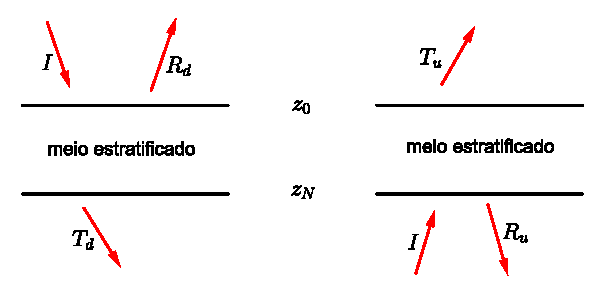
\includegraphics[scale=1.6]{ondas_ascen_descen}
%\caption{\textit{Dire\c{c}\~ao e sentido de propaga\c{c}\~ao de ondas ascendentes e descendentes em camadas homog\^eneas.}}
%\label{fig.ondas_ascen_descen}
%\end{figure}
%Vamos usar a const\^ancia da fun\c{c}\~ao dada na equa\c{c}\~ao \ref{eq.G(V,W)} para igualar seus valores calculados no topo e no fundo da pilha de camadas. Mas aqui, vamos tomar as ondas $V$ e $W$ com for\c{c}a $I$ em sentido descendente e ascendente, respectivamente.  
%\begin{equation*}
%\begin{bmatrix}
%R_d^\top&I
%\end{bmatrix}
%\begin{bmatrix}
%0&I\\
%-I&0
%\end{bmatrix}
%\begin{bmatrix}
%T_u\\
%0
%\end{bmatrix}
%=
%\begin{bmatrix}
%0&T_d^\top
%\end{bmatrix}
%\begin{bmatrix}
%0&I\\
%-I&0
%\end{bmatrix}
%\begin{bmatrix}
%I\\
%R_u
%\end{bmatrix}\,,
%\end{equation*}
%de onde conclu\'imos que
%\begin{equation}\label{eq.T}
%T_u=T_d^\top\,.
%\end{equation}
%Podemos ainda calcular o valor da fun\c{c}\~ao usando somente ondas descendentes $G(V,V)$. Igualando seus valores para o topo e a base da pilha de camadas, temos
%\begin{equation*}
%\begin{bmatrix}
%R_d^\top&I
%\end{bmatrix}
%\begin{bmatrix}
%0&I\\
%-I&0
%\end{bmatrix}
%\begin{bmatrix}
%R_d\\
%0
%\end{bmatrix}
%=
%\begin{bmatrix}
%0&R_d^\top
%\end{bmatrix}
%\begin{bmatrix}
%0&I\\
%-I&0
%\end{bmatrix}
%\begin{bmatrix}
%I\\
%R_d
%\end{bmatrix}\,,
%\end{equation*}
%de onde conclu\'imos que 
%\begin{equation}\label{eq.R_d}
%R_d=R_d^\top\,.
%\end{equation}
%Analogamente, para ondas ascendentes $G(W,W)$, temos \begin{equation}\label{eq.R_u}
%R_u=R_u^\top\,.
%\end{equation}
%Utilizando as equa\c{c}\~oes \ref{eq.T}, \ref{eq.R_d} e \ref{eq.R_u}, podemos definir uma matriz $R$ onde as componentes representam todas as ondas refletidas e transmitidas,
%\begin{equation*}
%R=
%\begin{bmatrix}
%R_d&T_u\\
%T_d&R_u
%\end{bmatrix}\,,
%\end{equation*}
%e verificar que 
%\begin{equation*}
%R=R^\top\,.
%\end{equation*}
%A matriz $R$ est\'a relacionada \`a matriz $S$ usada em \textit{Teoria de Dispers\~ao} de ondas,
%\begin{equation*}
%S=
%\begin{bmatrix}
%T_d&R_u\\
%R_d&T_u
%\end{bmatrix}\,,
%\end{equation*}
%e a matriz $S$ relaciona, de forma linear, ondas saindo de uma pilha de camadas com ondas entrando na pilha,
%\begin{equation*}
%\begin{bmatrix}
%\mathbf{D}(z_N)\\
%\mathbf{U}(z_0)
%\end{bmatrix}
%=
%S(z_0,z_N)\,
%\begin{bmatrix}
%\mathbf{D}(z_0)\\
%\mathbf{U}(z_N)
%\end{bmatrix}\,.
%\end{equation*} 
%
%\subsection{Rela\c{c}\~ao das Matrizes de Transmiss\~ao e Reflex\~ao com a matriz de Propaga\c{c}\~ao}
%
%As matrizes de reflex\~ao e transmiss\~ao podem ser escritas em termos das submatrizes da matriz de propaga\c{c}\~ao, da seguinte forma:
%\begin{align}\nonumber
%T_u(z_0,z_N)&=Q_{11}^{-1}(z_N,z_0)\,,\\\nonumber
%R_u(z_0,z_N)&=Q_{21}(z_N,z_0)\,Q_{11}^{-1}(z_N,z_0)\,,\\\label{eq.relacao_Q_R_T}
%R_d(z_0,z_N)&=-Q_{11}^{-1}(z_N,z_0)\,Q_{12}(z_N,z_0)\,,\\\nonumber
%T_d(z_0,z_N)&=Q_{22}(z_N,z_0)-Q_{21}(z_N,z_0)\,Q_{11}^{-1}(z_N,z_0)\,Q_{12}(z_N,z_0)\,,
%\end{align}
%e a matriz de propaga\c{c}\~ao \'e dada em fun\c{c}\~ao das matrizes de reflex\~ao e transmiss\~ao por
%\begin{equation*}
%Q(z_0,z_N)=
%\begin{bmatrix}
%T_u^{-1}&-T_u^{-1}R_d\\
%R_uT_u^{-1}&T_d-R_uT_u^{-1}R_d
%\end{bmatrix}\,.
%\end{equation*}
%
%
%Para o caso de camadas homog\^eneas, usando as equa\c{c}\~oes \ref{eq.Q(z,z_0)} e \ref{eq.relacao_Q_R_T}, podemos deduzir que, para matrizes de transmiss\~ao,
%\begin{equation*}
%T_d(z_0,z)=T_u(z_0,z)=\exp\left[\pm i\omega\,\Lambda(z-z_0)\right]\,,
%\end{equation*}
%e para matrizes de reflex\~ao
%\begin{equation*}
%R_d(z_0,z)=R_u(z_0,z)=0\,.
%\end{equation*}
%
%Vamos definir $E_{k+1}(-\pm i\omega)=\exp\left[-\pm i\omega\,\Lambda(z_{k+1}-z_k)\right]$. Assim, a matriz $S$ para uma camada homog\^enea e para interface para a pr\'oxima camada \'e dada pelo \textit{produto estrela},
%\begin{align*}
%S(z_{k+},z_{k+1+})&=S(z_{k+},z_{k+1-})*S(z_{k+1-},z_{k+1+})\\\\
%&=
%\begin{bmatrix}
%E_{k+1}(-\pm i\omega)&0\\
%0&E_{k+1}(-\pm i\omega)
%\end{bmatrix}
%*
%\begin{bmatrix}
%T_{d,k+1}&R_{u,k+1}\\
%R_{d,k+1}&T_{u,k+1}
%\end{bmatrix}\\\\
%&=
%\begin{bmatrix}
%T_{d,k+1}E_{k+1}(-\pm i\omega)&R_{u,k+1}\\
%E_{k+1}(-\pm i\omega)R_{d,k+1}E_{k+1}(-\pm i\omega)&E_{k+1}(-\pm i\omega)T_{u,k+1}
%\end{bmatrix}\,.
%\end{align*}